\chapter{Methods}
\label{chap:method}
 The approach we use for improving automatic playtesting can be divided into three major stages:
 \begin{enumerate}
    \item \textbf{Player modeling.} In this first stage, we model different cohorts of players based on their features. Furthermore, we create artificial agents that simulate their strategies in the game. Since we use human gameplay data to learn the strategies, using the taxonomy defined in \cite{yannakakis_player_2013}, we can classify our method as a direct modeling approach. However, since we do not have any direct strategy feature, we use unsupervised learning techniques in this stage. To model the players we evaluate the following two approaches:
     \begin{enumerate}
        \item \textbf{Clustering players.} First we cluster the players and then we train a different \acs{CNN}-based agent on each player cluster.

        \item \textbf{Clustering simulated strategies.} We train a \acs{CNN}-based agent feeding as input both the player features and the game board. Then, during prediction, by changing the players' input parameters, we can simulate several type of players. Lastly, clustering the simulated strategies we select different agents. 

     \end{enumerate}
    \item \textbf{Gameplay simulation.} On each level, various agents, simulating different player strategies, play the entire level several times. Based on the result of the simulation we compute the \acs{sr} of each agent.
    
    \item \textbf{Players' \acs{sr} prediction.} The final stage is to use the agents' SR on the training levels to fit a prediction model. Using this model we can predict the players' \acs{sr} on new levels.
\end{enumerate}

To perform automatic playtesting, the first stage is executed only one time or when major changes, that made the player models previously defined no longer reliable, are introduced in the game. On the contrary, stages two and three need to be performed each time a new generated game content needs to be tested.

 The novelty of these approaches relies in stage 1. Differently from existing approaches, we model strategies of various cohorts of players by directly learning them from player gameplay data. Some of the existing approaches for automatic playtesting consider only a single strategy while others, even if they simulate various strategies, rely on designers' knowledge or reinforcement learning to model them, without considering player data. Furthermore, to the best of our knowledge, this is the first attempt to use player modeling in a match-three puzzle game. In the next section, we describe the data used in our research. Then, we describe in detail the stages of our two approaches and the evaluation measures used. Finally, we propose an approach to estimate the strategy required by each level to be solved. 
 
\section{Data}
\subsection{Data Collection}
Since the number of daily active players for the \textit{Candy Crush Saga} game is large and the generated data is greater than what can be used as training data for a \acs{CNN}-based agent in a reasonable amount of time, we decided to track moves and players' statistics only from a subset of all the active players (\textasciitilde1\%). The tracking process of the moves lasted for three months collecting a good and diverse sample of player data. By contrast, the players' statistics, e.g. player's SR or number of boosters used, have been continuously collected while the player was playing the game. This allows to have accurate measures of the player behaviour not only on the levels played during the tracking period.
We collected data from level 1 to level 2945. Levels in the range [1, 2500] are used as training data for the player modeling stage, while levels in the range [2501, 2945] are used as test data in the players' \acs{sr} prediction stage. The split ensures that training data contains all the possible elements of the game since no item is introduced for the first time after level 2500. Furthermore, this split reproduces the same process that is performed in practice where existing levels are used as training data while predictions are performed on future ones. We remind that, as mentioned in Section \ref{delimitations}, we removed levels constrained by time or that contain the "Candy Frog" from the data set. Furthermore, due to an error in the game engine interface that is used by the agents to simulate gameplay in \textit{moves levels}, we removed also this type of levels. Nevertheless, these levels represent only 4.6\% of the total number of levels. This leads to 2161 training levels and 414 test levels.

\subsection{Data Representation}\label{data_representation}
\textbf{Game board features:} Each state is represented by 101 feature layers each one of size 9x9. The feature layers can be categorized into four main types:
\begin{enumerate}
    \item \textbf{Item layers.} There are 80 binary input layers that encode, with a binary representation, the items on the game board. Each of these layers is associated to a single item. Each position in the grid is set to 1 if the item is present and on the contrary, it is set to 0 if the item is not present. Since on each game board, only a subset of all the possible items is present, the layers associated with items that are not on the game board are filled with 0s.
    
    \item \textbf{Objective layers.} There are 19 binary feature layers of this type. Each layer represents a different objective that need to be achieved to win the level. It is filled with 1s if the objective is not yet fulfilled in the given state and contrarily it is filled with 0s if the objective is already fulfilled or if the objective is not requested for the given level.
    
    \item \textbf{Moves left layer.} A layer that represents the number of moves left to finish the level. In the game the maximum number of available moves is 75 and as a consequence the moves left can assume values in the range $\left[1,75\right]$. To give more importance to the last available moves we encode this feature as the ratio of 1 on the number of moves left. Adding this non-linearity has the effect of creating bigger changes in the feature when the moves available are only a few. A change of 1 move left when the available moves are few has a bigger impact on the feature rather than the same change of 1 move when the available moves are a lot. This is because if a player has 75 or 74 available moves he probably do not give too much importance to this difference while if he has only 1 or 2 available moves, the difference becomes important.
    
    \item \textbf{Bias layer.} Additionally, we stack a layer filled with all 1s. This layer allows the network to learn a bias on the position of the performed move in the grid. It is possible that moves in a specific area of the grid are preferred to moves in other positions. For example moves in the lower part of the board could be preferred to moves in the higher part because they increase the probability of creating cascade effects and obtaining more points. This layer can be described as an overall "heatmap" of the performed moves. It add a bias representing the likelihood of choosing a move in a specific position on the grid independently of the content of the game board.
\end{enumerate} 
Note that except for the item layers, the other layers encode only a single value. As a consequence the layers are created by repeating the value in every cell of the 9x9 plane. This allows to exploit the properties of the convolutional neural network also for this input information. \\

\noindent
\textbf{Moves:}
 Each move is a swap between two candies or items. By enumerating the inner edges of the game grid we encode the moves with a scalar number.  As showed in Figure \ref{fig:moves_encoding}, the moves are encoded enumerating first all the horizontal edges and then all the vertical ones. Since the cases where the direction of the move has an impact on the game are rare, we decided to do not distinguish between left-right or right-left moves and between top-down or bottom-up moves. This leads to a total number of 144 possible moves represented with integer values in the range [0, 143]. \\
 \begin{figure}[h!]
    \centering
    \resizebox{0.4
\textwidth}{!}{%
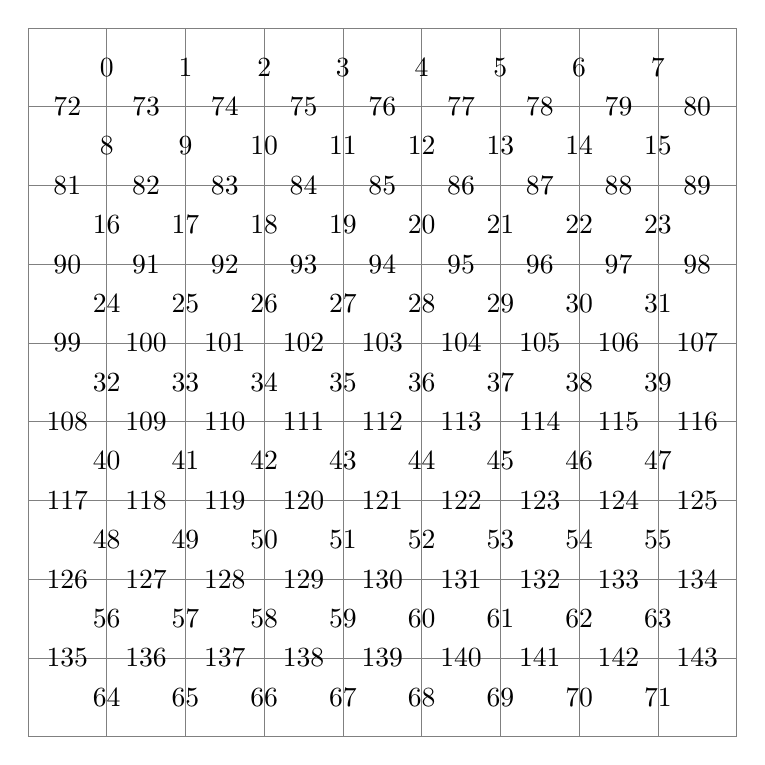
\begin{tikzpicture}[]
\draw[step=1cm,gray,very thin] (0,0) grid (9,9);

\foreach \x in {1,2,3,4,5,6,7,8}{
    \foreach \y [evaluate=\y as \index using int(\x-1+(\y-1)*8)] in {1,2,3,4,5,6,7,8,9}{
        \node at (\x, 9.5 - \y) {\index};
    }
}

\foreach \x in {1,2,3,4,5,6,7,8,9}{
    \foreach \y [evaluate=\y as \index using int(71+\x+(\y-1)*9)] in {1,2,3,4,5,6,7,8}{
        \node at (\x - 0.5, 9-\y) {\index};
    }
}

\end{tikzpicture}
}
    \caption{Moves encoding. Adapted from \cite{eisen_simulating_2017}.}
    \label{fig:moves_encoding}
\end{figure} 

\noindent
\textbf{Player features:}
In Table \ref{tab:player_features} we list all the per-level player features that we use to explore the differences in the player strategies. 
We define as an attempt each trial to solve a level. An attempt is considered ended if the player completes all the objectives, ends all the available moves or decides to exit the level. If a player decides to use a booster that adds extra moves, the attempt ends when also all the extra moves are terminated.  
An attempt is considered ended with a success if the player is able to achieve all the objectives within the constraints of that specific level. Since in this work we do not focus on the subset of levels that have time requirements, the constraint is always a maximum number of moves the player can use to complete the level. As boosters, we consider all the possible types: pre-level, in-level and consolation boosters. Each extra move is considered as a single booster. For example, a plus five extra moves is counted as five boosters. 
\begin{table}[ht]
    \centering
    \small
    \caption{Player features per level}
    \begin{tabular}{l}
    \toprule

    Features \\
    
    \midrule
    % Number of attempts ended \\
    % Number of attempts ended with success \\
    % Number of attempts started \\
    % Maximum number of stars \\
    % Maximum score \\
    % Number of boosters used \\
    Number of attempts ended\\
    Number of attempts ended with success \\
    Number of boosters used \\
    \bottomrule
        
    \end{tabular}
    \label{tab:player_features}
\end{table}

\section{Player Modeling}
The first stage aims to model players with different strategies. The goal of this stage is to generate multiple agents that simulate different strategies instead of having a single model that only simulates an average strategy learnt from all the players. Notice that the strategy learnt by the baseline approach is a combination of examples collected randomly from all the players. As a consequence it only represents an average strategy but it does not represent the strategy of an average player. Since for each player we have the performed moves in different states, a direct comparison between gameplay data cannot tell us how differently the players play. In the following, we describe the two different approaches we introduce for modeling various strategies while learning them directly from player data. 


\subsection{Clustering Players Approach}
The idea is to cluster the players into different groups based on their performance in the game. A first objective with this approach is to discover if players with different performances in the game exhibit a different decision making tendency or strategy and if a \acs{CNN}-based agent is able to capture it, approximating a policy function that shapes their actions in the game. This approach consist of three major stages:
\begin{enumerate}
    \item Computing player metrics
    \item Clustering players
    \item Training of \acs{CNN}-based agents
\end{enumerate}

\paragraph{1. Computing player metrics:}
Using the collected player features, for each player we compute the success rate $sr_i$, on each level $i$, as follows:
\begin{equation}\label{sucess_rate_i}
      sr_i  = \frac{s_i}{a_i} \text{,}
\end{equation}
where $s_i$ is the total number of attempts ended with a success and $a_i$ is the total number of attempts started by the player on level $i$. 
% We decided to use the number of attempt started, to consider as a failed attempts also when a player close the game while he is playing.
Using the per-level SR, we can represent each player with a one dimensional array containing all his SR ordered from level 1 to the last level played by each player. Due to privacy reasons we cannot expose the actual players' SR and as a consequence we use the standardized success rate $\rho_i$ computed as:
\begin{equation}\label{standardized_sr}
       \rho_{i}  = \frac{sr_i - \mu_i }{\sigma_i} \text{,}
\end{equation}
where $\mu_i$ is the average and $\sigma_i$ is the standard deviation of the $SR$ between all the players on level $i$.
An alternative to describe the players, could be to use the maximum number of stars or the maximum score on each level. However, the number of stars can assume only three values while the maximum score contains several outliers. As a consequence, we decided to use the players' SR to more accurately describe the player performances on each level.
Furthermore, in order to have a fair and complete comparison between players, in this approach we restrict our scope only to those players who finished all the training levels. In other words, we eliminate players that did not reach level 2500. This lead to a subset of $32,479$ players. This is also motivated by the fact that we are interested in predicting the perceived difficulty only on new levels and in order to play these levels, a player must have finished all the previous ones. We remind that we tracked only approximately 1\% of the total number of active players.

\paragraph{2. Clustering players:}
Using k-means with euclidean distance we cluster the players' SR distributions to create $k$ clusters of players with similar skill distributions over the training levels. We use k-means since it can work with data with high dimensionality and euclidean distance. Furthermore, k-means computes centroids that can give us a qualitative interpretation of what kind of player group each cluster represents. In order to decide the number of player clusters, represented by the parameter $k$, we use the elbow criterion.

\paragraph{3. Training of \acs{CNN}-based agents:}
Coherently with the defined player clusters, we divide the state-action pair represented by the game boards and the associated performed moves. As a consequence, each cluster data set contains moves tracked from players with similar skill distributions. Then, on each cluster, we train a \acs{CNN} that given the game board as input, predicts the performed move of the player. All the agents are trained for 10 epochs with the same network architecture and the same hyperparameters. For each agent we use 30 million state-action pairs randomly selected from each cluster data set. The test sets consist of 100,000 state-action pairs for each cluster. The training takes about 18 hours on a single machine with 6 CPUs and one Nvidia Tesla K80 GPU. Figure \ref{fig:clustering_players_flow} summarize the various steps of this approach. \\

Finally, as a baseline for this approach, we train an identical \acs{CNN}-based agent with the same amount of data and for the same amount of steps as each cluster agent. The gameplay data are randomly selected from data tracked from player that reached level 2500 without any distinction based on player features. 

\begin{figure}[!ht]
    \centering 
    \resizebox{0.8\textwidth}{!}{%
\begin{tikzpicture}[
decision/.style={diamond, draw, text width=4.5em, text badly centered, node distance=3.5cm, inner sep=0pt},
action/.style   ={rectangle, draw, text width=6em, text centered, rounded corners, minimum height=4em, minimum height=2em},
block/.style   ={rectangle, draw, text width=6em, text centered, rounded corners, minimum height=4em, minimum height=2em},
cloud/.style   ={draw, ellipse, minimum height=2em},
line/.style    ={draw,-latex'},
document/.style = {document, draw, text width=4em, text centered},
node distance=0.5cm, 
auto,]



% Define the nodes
\node[action]                            (dt)        {Tracking data};
\node[action,   right=of dt]             (pp)        {Computing player performance features};
\node[action,   right=of pp]             (cp)        {Clustering players};
\node[action,   right=of cp]             (cd)        {Creating training data sets};
\node[block,    above right=of cd,]      (dpc1)       {Data set from players in cluster 1};
\node[block,     right=of cd,]      (dpc2)       {Data set from players in cluster ... };
\node[block,    below right=of cd,]      (dpc3)       {Data set from players in cluster k};
\node[action,    right= of dpc2]     (tr)        {Training CNNs};
\node[block, above right = of tr]      (nn_1)     {Model trained on cluster 1};
\node[block,  right = of tr]      (nn_2)     {Model trained on cluster ... };
\node[block, below right = of tr]       (nn_3)     {Model trained on cluster k};


% % Connect the nodes
\path[line] (dt) -- (pp);
\path[line] (pp) -- (cp);
\path[line] (cp) -- (cd);
\path[line] (cd) -- (dpc1);
\path[line] (cd) -- (dpc2);
\path[line] (cd) -- (dpc3);
\path[line] (dpc1) -- (tr);
\path[line] (dpc2) -- (tr);
\path[line] (dpc3) -- (tr);
\path[line] (tr) -- (nn_1);
\path[line] (tr) -- (nn_2);
\path[line] (tr) -- (nn_3);



\end{tikzpicture}
}
    \caption{Clustering players flow: We track data from a subset of all active players. We then compute player performance features and we cluster the players into $k$ clusters. Then, we divide the data set based on the defined clusters. The generated data sets are then used to train $k$ different predictive models.}
    \label{fig:clustering_players_flow}
\end{figure}




\subsection{Clustering Simulated Strategies Approach}
The idea is to let the \acs{CNN} automatically discover the relationship between the player features and the performed moves since the neural network is able to automatically discover even complex relationships between input and output. Similarly to what \textcite{maddison_move_2014} did in their research, we provide the network with additional information regarding the player who performed the move. Compared to the previous approach, where we target one type of player at a time, it has the advantage of avoiding a substantial reduction of training data.
This approach consists of four major stages:

\begin{enumerate}
    \item Computing player metrics
    \item Training the \acs{CNN}-based agent
    \item Predicting moves simulating different players
    \item Clustering the simulated strategies
\end{enumerate}

\paragraph{1. Computing player metrics:}
Since we leave to the \acs{CNN} the task of learning the relationship between player features and predicted moves, this time we use three different dimensions to represent each player. \\
First of all, using the collected player features, we compute the standardized success rate $\rho_{i}$ on each level $i$ as defined in equation \ref{standardized_sr}. Similarly, we computed the average amount of boosters $b_i$, used on each level $i$, as follows:
\begin{equation}
      b_i  = \frac{\text{boosters}_i}{a_i} \text{,}
\end{equation}
where $\text{boosters}_i$ is the total number of boosters used by the player on level $i$ and $a_i$ is the total number of attempts started by the player on level $i$. Subsequently, we compute the standardized value $\beta_i$ as:
\begin{equation}
       \beta_i  = \frac{b_i - \mu_i }{\sigma_i} \text{,}
\end{equation}
where $\mu_i$ is the average and $\sigma_i$ is the standard deviation of the amount of boosters $b_i$ between all the players on level $i$.
Finally, for each player, we compute the following three summary statistics:
\begin{itemize}
    \item The standardized mean success rate $\bar{\rho}$ as:
        \begin{equation}
            \bar{\rho}  = \frac{1}{l} \sum_{i \in L} \rho_i \text{,}
        \end{equation}
    where $L$ is the subset of levels played by the player during the tracking period and $l$ is the number of levels in $L$.
    \item The standardized mean amount of booster $\bar{\beta}$, computed as:
        \begin{equation}
            \bar{\beta} = \frac{1}{l} \sum_{i \in L} \beta_i \text{,}
        \end{equation}
    where $L$ is the subset of levels played by the player during the tracking period and $l$ is the number of levels in $L$.
    \item The number of levels played $l$ during the tracking period.
    % computed as:
    %     \begin{equation}
    %         \lambda  = \frac{l - \mu }{\sigma} \text{,}
    %     \end{equation}
    % where $\mu$ is the average and $\sigma$ is the standard deviation of the number of levels $l$ played between all the players.
\end{itemize}
\noindent
These three player features can be joined together through a unique identifier that represents a specific player. For privacy concern, this unique identifier is anonymised in a way that is not possible to go back to the real player. We decided to use these three metrics because we believe that they can exhaustively represent the various types of players in the investigated game, e.g. skilled vs less skilled players or regular vs occasional players. Since we only take average values between all the levels played by a player, we do not anymore need to restrict our focus on players who completed all the $2,500$ training levels. 

Furthermore, standardizing the \acs{sr}, is not only necessary for privacy reasons but it also helps to take into account that different players may have played different levels. Computing the standard values includes the difficulty of each level in the player metric. However, in order to have meaningful summary statistics, we removed players who played less than 50 levels. This is motivated by the fact that the mean, if computed on few values, becomes too sensitive to outliers. Despite this, we still have tracked data from more than half a million players.


\paragraph{2. Training the \acs{CNN}-based agent:}
We train a \acs{CNN}-based agent that given the game board and the three player features as input, predicts the move performed by the corresponding player. Since players are not divided into groups, we have much more data compared to the previous approach. Therefore, the network is trained for 10 epochs using 125 million state-action pairs as training data. The training data are selected to have approximately 50,000 examples for each level in the range [1, 2500]. As a consequence, each level is represented with a similar amount of data. The training takes about 3 days on a single machine with 6 CPUs and one Nvidia Tesla K80 GPU. The test data consist of 100,000 examples.

\paragraph{3. Predicting moves simulating different players:}
The trained \acs{CNN} acts as a move predictor sensitive to player features. It is able to generate different player moves for the same input game board only by changing the input player parameters. The player features are continuous values and, in theory, we can simulate an infinite number of players. Since our goal is to generate a reasonable amount of different agents, we select for each player features the 5th, 25th, 50th, 75th and 95th percentile and we create an agent for each possible combination of these parameters. These percentiles are selected to have an extensive representation of the real players. We decided to not use the extreme values because they might represent anomalous players. 

Finally, each agent is created by cloning the trained \acs{CNN} and fixing the input player features with a combination among those selected. This generates 125 different agents, each one simulating a different type of player.

\paragraph{4. Clustering the simulated strategies:}
The 125 generated agents can be an exhaustive representation of the different type of players in the \textit{Candy Crush Saga} game. However, simulating gameplay of 125 agents for each level that needs to be tested is computationally expensive. Moreover, some of these agents simulate very similar strategies. In this step, we want to reduce the number of generated agents maintaining only a small number of agents while maximizing the differences in the simulated strategies. To select the agents, we create a validation data set with 10,000 state-action pairs and for each agent we predict the moves. We can then represent each agent with a one-dimensional array containing the predicted moves. Each array can be considered as an explicit representation of the strategy of each agent. Then, we use hierarchical clustering with hamming distance and complete-linkage function on the generated arrays, to group agents with similar strategies. Finally, we select a single agent for each cluster. Figure \ref{fig:clustering_simulated_strategies_flow} summarizes the various steps of this approach. \\

As a baseline for this approach, we train a \acs{CNN}-based agent for the same number of steps and using the exact same data but without the input player features. As a result, the baseline agent represents an average policy between all the players and simulates a single strategy. It is worth to remember that the objective of this thesis is not to directly compare the two experimented approaches, but to understand if each approach is better than its own baseline answering if player modeling can improve automatic playtesting.
 

\begin{figure}[ht!]
    \centering
    \resizebox{0.8\textwidth}{!}{%
\begin{tikzpicture}[
decision/.style={diamond, draw, text width=4.5em, text badly centered, node distance=3.5cm, inner sep=0pt},
action/.style   ={rectangle, draw, text width=6em, text centered, rounded corners, minimum height=4em, minimum height=2em},
block/.style   ={rectangle, draw, text width=6em, text centered, rounded corners, minimum height=4em, minimum height=2em},
cloud/.style   ={draw, ellipse, minimum height=2em},
line/.style    ={draw,-latex'},
document/.style = {document, draw, text width=4em, text centered},
node distance=0.5cm, 
auto,]



% Define the nodes
\node[action]                            (dt)        {Tracking data};
\node[action,   right=of dt]             (pf)        {Computing player features};
\node[action,   right=of pf]             (tr)        {Training CNN};
\node[action,   right=of tr]             (sf)        {Selecting player features};
\node[block,    above right=of sf,]      (ag1)       {Agent 1};
\node[block,     right=of sf,]      (ag2)       {Agent ... };
\node[block,    below right=of sf,]      (ag3)       {Agent 125};
\node[action,    right= of ag2]     (pr)        {Predict moves on validation set};
\node[action,    right= of pr]     (css)        {Clustering simulated strategies};
\node[block, above right = of css]      (nn_1)     {Model 1};
\node[block,  right = of css]      (nn_2)     {Model ... };
\node[block, below right = of css]       (nn_3)     {Model k};


% % Connect the nodes
\path[line] (dt) -- (pf);
\path[line] (pf) -- (tr);
\path[line] (tr) -- (sf);
\path[line] (sf) -- (ag1);
\path[line] (sf) -- (ag2);
\path[line] (sf) -- (ag3);
\path[line] (ag1) -- (pr);
\path[line] (ag2) -- (pr);
\path[line] (ag3) -- (pr);
\path[line] (pr) -- (css);
\path[line] (css) -- (nn_1);
\path[line] (css) -- (nn_2);
\path[line] (css) -- (nn_3);



\end{tikzpicture}
}
    \caption{Clustering simulated strategies flow: We track data from a subset of all the active players. We then compute player features and we train a \acs{CNN}-based agent giving as input the game board and the player features. Then, we predict moves on a validation set with different agents. Each agent shares the same network but it has a different player input feature combination. Finally, we cluster the simulated strategies and we select the agents maximizing the differences in their predictions.}
    \label{fig:clustering_simulated_strategies_flow}
\end{figure}


\section{Gameplay Simulation}
\textcite{eisen_simulating_2017} illustrated how a \acs{CNN}-based agent can be used to predict human moves in the \textit{Candy Crush Saga} game. Since his approach reached the best performance to date, we decided to use a similar network architecture for predicting player moves. 

\subsection{Player Moves Prediction}
%After the successful results in predicting expert moves in the game of \textit{Go} \cite{silver_mastering_2017}, 
This stage is identical for both the experimented approaches since it does not depend on how we created the various agents. To simulate gameplay, for each agent, we use the following infrastructure. Several machines run the game engine, integrated with the agent interface, that takes care of simulating the attempts. At the same time, on a web server we run various replicas of the \acsp{CNN}. We decided to separate these two components to allow the agent to use different approaches to select the moves, abstracting it from the predictions of the neural network. The agent interfaces communicate with the \acsp{CNN} trough a component called load balancer. The main task of the load balancer is to redirect the requests received from the agent interfaces to the \acs{CNN} with the lowest utilization. The requests contain the encoded game state obtained from the agent. The response is the predicted probability distribution over the 144 possible moves. When an attempt is finished, the results of the simulation are saved on a table using MySQL database.

For each agent we ran a simulation on both training and test levels. A simulation consists of 100 attempts on each level. This number is selected to run the simulation in a reasonable amount of time. Each attempt runs with a different seed that causes the game to generate different random content. However, to have a fair comparison between agents, the selected seeds are the same for each simulation. The simulation takes approximately 18 hours for each agent while running on a total of 26 \acf{vCPU} cores and 24 GB of memory. The \acs{vCPU} cores are divided between the various components as follow: 18 \acs{vCPU} cores are used to run the bot interface, 2 \acs{vCPU} cores are used by the load balancer while the remaining 6 \acs{vCPU} cores are used to run the \acsp{CNN}. This allocation of resources has demonstrated to work well in practice, in term of speed and utilization. All the computational resources are allocated using a cloud service provider.
When the network is used as an agent to simulate gameplay, a greedy policy is used to select the moves. Since the output of the network is a probability distribution over the 144 available moves, the greedy policy selects the move with the highest predicted probability. 
% Only in the unusual case in which the greedy move is not a legal one, in order to progress in the gameplay simulation, we select the legal move with the highest predicted probability. 
Finally, from the results of the simulations we compute the agents' \acs{sr} on each level. These metrics indicate how difficult a level is for each agent.


\subsection{Convolutional Neural Network Architecture}
When designing a \ac{CNN}, several architectural choices need to be taken and various hyperparameters need to be selected. In this research we rely on the choice made and discussed in \cite{eisen_simulating_2017} with only small changes to the input layer to consider the player features in the clustering simulated strategies approach. For completeness, in this section, we describe the network architecture used for predicting the moves given the states. The network, illustrated in Figure \ref{fig:network_architecture}, is trained with Adam optimizer \cite{kingma_adam:_2014} and an initial learning rate of 0.0005.

\paragraph{Input Layer:}
The input of the network slightly differs between the two approaches we illustrate in our research. In the clustering players approach, the input is represented by 101 layers each one of size 9x9 to represent a game board as described in Section \ref{data_representation}. To train the network we use mini-batch gradient descent with a batch size of 2048 examples since it showed to be a good compromise between accuracy and efficiency. This lead to an input of size [2048x9x9x101]. Differently, in the clustering simulated strategy approach, we add as input three player features leading to an input size of [2048x9x9x104].

\paragraph{Convolutional Layers:}
The network consists of 11 convolutional layers with 35 filters per layer and kernel size of 3x3. Since we do not want the translation invariance property of \acs{CNN} architectures because we want to accurately determine which move to select, we do not use pooling layers. Furthermore, since the game board is only 9x9, we want the output size to be the same as the input size. As a consequence, we used zero-padding and filters with stride of 1.
Subsequently, a last convolutional layer with 144 filters is added to the network. The range $\left[0,143\right]$ represents the encoding of the 144 possible moves that the network can predict.
Each convolutional layer is followed by an \acf{ELU} activation function. The \acs{ELU} function, introduced by \textcite{clevert_fast_2015}, is computed as follow:
\begin{equation}
    f(x)= 
            \begin{cases}
                x,                 & \text{if } x > 0\\
                \alpha (e^x-1),     & \text{if } x \leq 0  
            \end{cases}
\end{equation}
where the \acs{ELU} hyperparameter $\alpha$ controls the saturation of the \acs{ELU} function for negative values. As suggested in \cite{clevert_fast_2015}, we use a value of $\alpha=1.0$. Compared to \acf{ReLU} function, the \acs{ELU} function has also negative values, which allow the network to push the mean of each activation map closer to zero, reducing the \textit{bias shift} typical of \acs{ReLU} functions. Furthermore, as showed in \cite{eisen_simulating_2017}, the \acs{ELU} improved the accuracy of the model by 2.5\% compared to the \acs{ReLU} function.  

\paragraph{Output Layer:}
The output layer is a \acs{GAP} layer that transforms the 144 activation maps of the last convolutional layers into 144 scalars retaining only the average value for each map. Using a \acs{GAP} layer also motivates the choice of encoding the information represented by scalar values into feature planes by replicating the number on all the cells of the 9x9 grid. Otherwise a fully connected layer would be necessary to include these features into the model. Finally, in order to have a probability distribution over the predicted moves, the \textit{softmax} function is applied.

\begin{figure}
    \centering
    \resizebox{\textwidth}{!}{%
\begin{tikzpicture}[
decision/.style={diamond, draw, text width=4.5em, text badly centered, node distance=5cm, inner sep=0pt},
action/.style   ={rectangle, draw, text width=6em, text centered, rounded corners, minimum height=4em, minimum height=2em},
block/.style   ={rectangle, draw, text width=7em, text centered,minimum height=2em, node distance=1cm,},
cloud/.style   ={draw, ellipse, minimum height=2em},
scalar_op/.style   ={text width=6em, text centered, minimum height=2em, node distance=1cm,},
half_scalar_op/.style   ={text width=1em, text centered, minimum height=2em, node distance=0.5cm,},
line/.style    ={draw,-latex'},
document/.style = {document, draw, text width=4em, text centered},
node distance=0.5cm, 
auto,]% Define the nodes
\node [scalar_op] (i) {input};
\node[block, right=of i, ] (c1) {3x3 conv,\\35 filters,\\ELU activation};
\node[below=of c1, shift={(0,5mm)}]{x11};
\node[block, right=of c1, ] (c12) {3x3 conv,\\144 filters,\\ELU activation};
\node[block, right=of c12, ](avg){global average pooling};
\node[block, right=of avg](sm){softmax};
\node[scalar_op, right=of sm](out){output};
%
%\draw[decorate,decoration={mirror,brace,amplitude=5pt,raise=50pt},yshift=10pt,yshift=0pt,-]
%  ([yshift=.5cm]c1.center) -- ([yshift=-.5cm]c11.center) node[black,midway,xshift=-70pt,rotate=90] (convlayers) {11 conv layers zero-padding to maintain dimensions};

%
%% Connect the nodes
\path (i) edge [->] (c1)
(c1) edge [->] node {} (c12)
(c12) edge [->] node {} (avg)
(avg) edge [->] (sm)% 
(sm) edge [->] (out);% 

%% draw cubes 
\pic at ([yshift=3cm]i.center) {annotated cuboid={width=9, height=9, depth=101, scale=.04, units=}}(a);
% 
\pic at ([yshift=3cm, xshift=0.5cm]c1.center) {annotated cuboid={width=9, height=9, depth=35, scale=.04, units=}}(b);
% \pic at ([xshift=3cm]inter.center) {annotated cuboid={width=9, height=9, depth=35, scale=.04, units=}}(c);
%%  \pic at ([xshift=3cm]c11.center) {annotated cuboid={width=9, height=9, depth=35, scale=.04, units=}}(c);
%
% 
\pic at ([yshift=3cm, yshift=-.5cm]c12.center) {annotated cuboid={width=9, height=9, depth=144, scale=.04, units=}};


%
%% draw vectors 
%\path ([xshift=2.5cm]l.center) edge [below,|-|] node {144} ([xshift=6cm]l.center);
%
\path ([xshift=-0.5cm,yshift=1.7cm]avg.center) edge [below,|-|] node[shift={(3mm,0)}] {144} ([yshift=4.2cm, xshift=1.8cm]avg.center);
\path ([xshift=-0.5cm,yshift=1.7cm]sm.center) edge [below,|-|] node[shift={(5mm,0)}] {144} ([yshift=4.2cm, xshift=1.8cm]sm.center);
\path ([xshift=-0.5cm,yshift=1.7cm]out.center) edge [below,|-|] node[shift={(5mm,0)}] {144} ([yshift=4.2cm, xshift=1.8cm]out.center);

 
% % Connect the cubes with arrows
% \path ([xshift=3cm, yshift=-1cm]i.center) edge [right,->] ([xshift=3cm, yshift=1cm]c11.center);

% \path ([xshift=3cm, yshift=-1cm]c11.center) edge [right,->] ([xshift=3cm,yshift=.2]c12.center);

% \path ([xshift=3cm, yshift=-1.5cm]c12.center) edge [right,->] ([xshift=3cm,yshift=-13]avg.center);

% \path ([xshift=3cm,]l.center) edge [right,->] ([xshift=3cm,yshift=0.2cm]sm.center);

\end{tikzpicture}
}
%    \input{contents/03_method/i00_network_architecture_horizontal}
    \caption{Convolutional neural network architecture used in the clustering players approach, with data representations for each layer. In the clustering simulated strategies approach, the input layer changes from 101 to 104 input features. Image generated with code adapted from \cite{eisen_simulating_2017}.} 
    \label{fig:network_architecture}
\end{figure}


\section{Players' SR Prediction}
At this step we have the per-level agents' \acs{sr} on both training and test levels. As demonstrated in \cite{eisen_simulating_2017}, the agents' \acs{sr} does not directly map to the \acs{sr} of the players. However, they are correlated. In this stage we combine the agents' \acs{sr} on test levels to better predict the players' \acs{sr} compared to the baseline in each of the two approaches. In order to not expose the actual values of the players' \acs{sr} for privacy reasons, we scaled the players' \acs{sr} dividing each value by the difference between the maximum and the minimum value.
As a consequence, the scaled players' success rate $sr_i^\prime$ on level $i$ is defined as:
\begin{equation}\label{eq:scaled_sr}
    sr_i^\prime = \frac{sr_i}{max(sr_i) - min(sr_i)} \text{,}
\end{equation}
where $sr_i$ is the actual players' success rate on level $i$, $max(sr_i)$ is the maximum success rate and $min(sr_i)$ is the minimum success rate between all the levels. This has the effect of scaling the values while maintaining the same distribution.
Furthermore, since the distributions of \acs{sr} for both the players and the agents have a positive skew, meaning that the mass of the distribution is concentrated on the left, we apply a log transformation on each variable. Nevertheless, applying the log transformation causes the values of the \acs{sr} that were zero to become minus infinite. As a consequence, we decided to use the mean value to predict the players' \acs{sr} when the agent's \acs{sr} is zero. An alternative could be to use the $log(x + 1)$ transformation where in our case $x$ is the agent's \acs{sr}. However, we prefer to handle the levels where the agent failed in a different way because when the agent's \acs{sr} is zero does not necessary mean that the level is extremely difficult. This is also motivated by the fact that for extremely low values of the agents' \acs{sr} there is no linear relationship with the players' \acs{sr}. Since levels are designed and tested to be solvable by humans within a reasonable number of attempts, extremely low values of the players' \acs{sr} do not exist. This explains why there is no linear relationship between extremely low values of the log of the players' and the log of the agents' \acs{sr}. We excluded those levels where all the agents and the baseline failed since they would just introduce noise to the comparison of the approaches. Finally, we decided to not use a cross-validation approach for two reasons: first, because we want to produce the same scenario that would be used in practice where the existing levels are used to make predictions on new levels and second because we trained the agents on the training levels only and we let them play on new ones to reduce overfitting. 
In this stage we use two slightly different methods for the two experimented approaches. 

\subsection{Clustering Players Approach}
Using the players' and agents' \acs{sr} on training levels we fit a linear regression model for each agent, including the baseline. Then, we use the linear models to predict the players' \acs{sr} on the test levels. 
An issue we need to take into account is that in \textit{Candy Crush Saga}, levels might have been modified during time. Since the players' \acs{sr} is computed from the players' attempts at the time they have played while the agents simulate the current version of the levels, we eliminate from our data set those levels that have drastically changed. We classify a modified level as drastically changed if the players' \acs{sr} on it changes more than $50\%$. These levels represent 18\% of the total number of levels and removing them leads to 1722 training levels and 388 test levels. 

Each model predicts the players' \acs{sr} of the specific group $k$ that it represents. In order to compare our approach with the state-of-the-art, we combine the predictions of the agents on each test level $i$, computing the overall predicted success rate $\widehat{sr}_i$ between all the players using a weighted average as follow:
\begin{equation}\label{combination}
    \widehat{sr}_i = \sum_{j = 1}^{k} w_j \cdot \widehat{sr}_{i,j} \text{,}
\end{equation}
where $k$ is the number of defined agents, $w_j$ is the percentage of players in cluster $j$ and $\widehat{sr}_{i,j}$ is the success rate on level $i$ of the agent trained with data from cluster $j$.
The idea is that the predictions of each agents have a weight that depends on the percentage of players that the agent simulates.
Finally, the predictions of this model are compared to the predictions of the linear regression model created from the baseline agent's \acs{sr}.

\subsection{Clustering Simulated Strategies Approach}

Since we cannot precisely determine how many players each agent represents, in this approach we predict on each test level $i$, the overall predicted success rate $\widehat{sr}_i$ between all the players using a single linear regression model. The model takes as input all the $k$ agents' success rates $\widehat{sr}_{i,j}$. The predictions of this model are then compared to the predictions of a linear regression model trained with the baseline agent's \acs{sr}. 


\section{Evaluation Metrics}

In this section we describe the metrics we use to evaluate both the move prediction performance of the \acs{CNN} models as well as the \acs{sr} estimation performance of the linear regression models.

\subsection{Player Moves Predictions}
To evaluate the performances of the \acs{CNN}-based agents in predicting player moves we use the top-1 and top-3 prediction accuracy. The top-1 and top-3 prediction accuracy are the ratios of correct predictions to the total number of predicted actions. However, the top-1 accuracy considers a prediction as correct if the correct move coincides with the predicted one while the top-3 accuracy considers a prediction as correct if the right move appears in the top three predicted ones.

\subsection{Linear Regression Models}
To compare the baseline agent with our approach, we compute three different measures. The goal is to see how close the predictions of each approach are to the actual observed values compared to the baseline. The measures used in this research are: the \acf{MAE}, the \acf{MSE} and the adjusted R-squared ($\text{R}^2_{adj}$).
The \acs{MAE} describes the means of the absolute differences between the predicted and the observed players' \acs{sr} on all the $n$ test levels and it is defined as:
\begin{equation}
    \text{MAE} = \frac{1}{n} \sum_{i=1}^{n} |\widehat{sr}_i - {sr}_i| 
\end{equation}
The \acs{MSE} measures the mean of the squared differences between the predicted and the observed players' \acs{sr} on all the $n$ test levels and it is defined as:
\begin{equation}
    \text{MSE} = \frac{1}{n} \sum_{i=1}^{n} (\widehat{sr}_i - {sr}_i)^2
\end{equation}
The \acs{MSE} has the property of strongly penalizing large deviations from the observed values.
Finally, the adjusted R-squared, explains the predictive power of the regression models considering the number of predictors. It decreases when a predictor improves the model less than what would be improved by chance. This is a desirable property since in the clustering simulated strategies approach, we compare a method that uses multiple predictors with the baseline approach that only uses a single predictor. The adjusted R-squared is defined as:
\begin{equation}
    \text{R}^2_{adj} = 1 - [\frac{(1-R^2)(n-1)}{n-k-1}] \text{,}
\end{equation}
where $n$ is the number of data points, $k$ is the number of predictors excluding the constant and $\text{R}^2$ equals the square of the Pearson correlation coefficient \cite{benesty_pearson_2009} between the observed and the predicted values.


\section{Estimating Strategy Requirements}

Finally, we aim to categorize levels based on the strategy required to solve them.
Similarly to what \textcite{isaksen_simulating_2017} have done with a simplified version of \textit{Tetris} and \textit{Puzzle Bobble}. First, they trained an agent that reached super-human performances in the two simplified games. Then they generated a population of different agents that play with slightly different heuristics and finally they made the agents more human-like by adding, in different quantities, two types of human errors: strategy and dexterity errors. A strategy error means that a human player not always selects the optimal move, sometimes he makes a mistake and he selects a sub-optimal or random move. A dexterity error means that even if the player knows which move he want to perform, sometimes he is not able to correctly perform it due to pressure, time-constraints or other limitations. 
This approach for player modeling is based on the idea that models of players are obtained from a super-human agent by adding human errors to it.
Using \textit{Candy Crush Saga} as a test bed we aim to estimate the impact of human errors on some levels. However, the motor-skill required to correctly perform a move in \textit{Candy Crush Saga} is very low and levels that require a lot of dexterity do not exist. As a consequence, we only focus on estimating the strategy requirement. Nevertheless, if the proposed approaches are applied to other games it may be valuable to estimate the dexterity requirement too. 
Since the variants of the games tested by \citeauthor{isaksen_simulating_2017} are small enough to evaluate the full game tree, they used heuristics and search to train the policy of the agents and they modeled human errors using variants of Q-learning. On the contrary, we propose an approach that works with \acs{CNN}-based agents and with more complex games. 
We model the strategy errors using a parameter $\epsilon$. We modify the policy of the agents from a greedy one to an $\epsilon$-greedy policy. Using an $\epsilon$-greedy policy means that the agent selects greedy moves with probability $1 - \epsilon$, while with probability $\epsilon$, the agent selects a random move with uniform distribution over the set of available moves. Selecting a greedy move means that we chose the move with the highest predicted probability from the \acs{CNN}-based agent output. Selecting moves randomly instead of greedily represents the strategy error simulated by the agent. This approach is built on the assumption that the strategy learnt from player data is enough to solve the levels. To obtain a meaningful analysis we restrict our focus to those levels that are successfully solved by the agent when playing with no strategy errors, using the greedy policy. Then, by comparing the performances of the agents, we estimate the strategy required by each level. Starting from the previously developed agent that simulates an average strategy, we create a population of different agents by adding different amount of strategy errors. Finally, we randomly selected some levels to test this approach. 

Furthermore, in their research, \citeauthor{isaksen_simulating_2017} used an agent that is able to play with an optimal strategy when the strategy error is zero. Since the complexity of the game we focus on is much higher and the game is non-deterministic, that type of agent is not available. As a consequence, we consider the greedy policy as the optimal policy and the \acs{sr} reached by the greedy agent as the maximum \acs{sr}. We normalize the values dividing all the obtained \acs{sr} by that maximum \acs{sr}. By plotting the agent's \acs{sr} against the amount of strategy used, represented by $1 - \epsilon$, we observe how the \acs{sr} improves as we reduce the number of random moves made by the agent. Figure \ref{fig:extremes} shows the two extreme cases. On the left a level that does not require any strategy since independently from how many random moves are performed the level is solved. On the right a level that requires the optimal strategy because if any strategy error is made the \acs{sr} is zero. These two extreme cases are not present in the game but are useful to give an idea of how to interpret the generated graphs.

Finally, to estimate the strategy required by a level, we compute the area above the line. This metric indicates how much strategy is required to complete the level. In the two extreme cases, the area above the line is zero when no strategy is required and it is one when the optimal strategy is needed.
\begin{figure}[h]
  \centering
  \subfloat[]{%No strategy required
    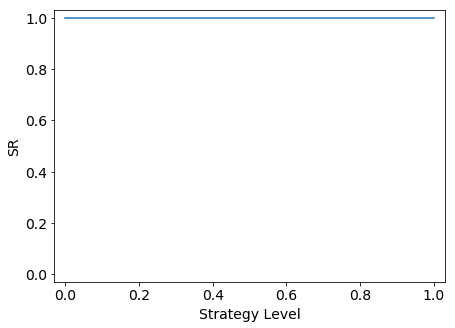
\includegraphics[width=0.45\textwidth]{masters-thesis-master/masters-thesis/contents/05_discussion/strategy_req/extreme2.png}
    \label{fig:extreme2}
    }
    \subfloat[]{%Full strategy required
    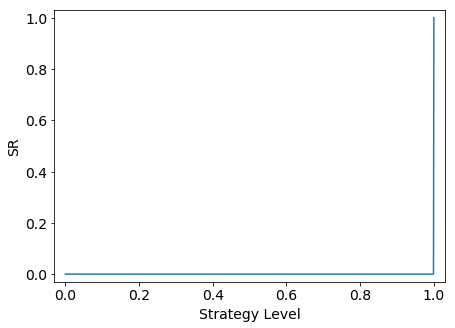
\includegraphics[width=0.45\textwidth]{masters-thesis-master/masters-thesis/contents/05_discussion/strategy_req/extreme1.png}
    \label{fig:extreme1}
    }
    
    \caption{Agent's \acs{sr} against strategy level for the two extreme cases of strategy requirements. Figure (a) shows a level that does not require any strategy while Figure (b) shows a level that requires 100\% of strategy in order to be solved.}
    \label{fig:extremes}
\end{figure}